%%%%%%%%%%%%%%%%%%%%%%%%%%%%%%%%%%%%%%%%%%%%%%%%%%%%%%%%%%%%%%%%%%%%%
%
% CSCI 1430 Written Question Template
%
% This is a LaTeX document. LaTeX is a markup language for producing documents. 
% You will fill out this document, compile it into a PDF document, then upload the PDF to Gradescope. 
%
% To compile into a PDF on department machines:
% > pdflatex thisfile.tex
%
% If you do not have LaTeX, your options are:
% - VSCode extension: https://marketplace.visualstudio.com/items?itemName=James-Yu.latex-workshop
% - Online Tool: https://www.overleaf.com/ - most LaTeX packages are pre-installed here (e.g., \usepackage{}).
% - Personal laptops (all common OS): http://www.latex-project.org/get/ 
%
% If you need help with LaTeX, please come to office hours.
% Or, there is plenty of help online:
% https://en.wikibooks.org/wiki/LaTeX
%
% Good luck!
% Srinath and the 1430 staff
%
%%%%%%%%%%%%%%%%%%%%%%%%%%%%%%%%%%%%%%%%%%%%%%%%%%%%%%%%%%%%%%%%%%%%%
%
% How to include two graphics on the same line:
%
% \includegraphics[width=0.49\linewidth]{yourgraphic1.png}
% \includegraphics[width=0.49\linewidth]{yourgraphic2.png}
%
% How to include equations:
%
% \begin{equation}
% y = mx+c
% \end{equation}
%
% How to include code:
%
% \begin{python}
% def f(x):
%   return x
% \end{python}
%
%
%%%%%%%%%%%%%%%%%%%%%%%%%%%%%%%%%%%%%%%%%%%%%%%%%%%%%%%%%%%%%%%%%%%%%%%%%%%%%%%%%%%%%%%%%%%%%%%%

% \documentclass[11pt]{article}

% \usepackage[english]{babel}
% \usepackage[utf8]{inputenc}
% \usepackage[colorlinks = true,
%             linkcolor = blue,
%             urlcolor  = blue]{hyperref}
% \usepackage[a4paper,margin=1.5in]{geometry}
% \usepackage{stackengine,graphicx}
% \usepackage{fancyhdr}
% \usepackage{amsmath}
% \usepackage{amssymb}
% \usepackage{enumerate}
% \setlength{\headheight}{15pt}
% \usepackage{microtype}
% \usepackage{times}
% \usepackage{booktabs}
% \usepackage[shortlabels]{enumitem}
% \setlist[enumerate]{topsep=0pt}
% \usepackage{mdframed}

% \usepackage{pythonhighlight}


% \frenchspacing
% \setlength{\parindent}{0cm} % Default is 15pt.
% \setlength{\parskip}{0.3cm plus1mm minus1mm}

% \pagestyle{fancy}
% \fancyhf{}
% \lhead{Homework 4 Questions}
% \rhead{CSCI 1430}
% % \lfoot{\textcolor{red}{Only 
% % \ifcase\thepage
% % \or instructions
% % \or A1
% % \or A1
% % \or A2
% % \or A2
% % \or Q3
% % \or A3
% % \or A4
% % \or A5
% % \or Q6
% % \or A6
% % \or Q7
% % \or A7
% % \or feedback
% % \else
% % EXTRA PAGE ADDED
% % \fi
% % should be on this page
% % }}
% \rfoot{\thepage~/ 14}

% \date{}

% \title{\vspace{-2cm}Homework 4 Questions}


% \begin{document}
% \maketitle
% \thispagestyle{fancy}
% \vspace{-3cm}

% \section*{Document Instructions}
% \begin{itemize}
%   \item 5 questions \textbf{[8 + 10 + 8 + 4 + 10 = 40 points]}.
%   \item Fill all your answers within the answer boxes, and \textbf{please do NOT remove the answer box outlines}.
%   \item Include code, images, and equations where appropriate.
%   \item To identify all places where your responses are expected, search for `TODO'.
%   \item Please make this document anonymous.
% \end{itemize}

% \section*{ Gradescope Instructions}
% \begin{itemize}
%   \item When you are finished, compile this document to a PDF and submit it directly to Gradescope. 
%   \item You will be required to assign the appropriate answers to the right pages on Gradescope. \textbf{Failure to assign pages correctly will lead to a deduction of 2 points per misaligned page (capped at a maxmimum 6 point deduction).}
% \end{itemize}
% \pagebreak




% % \paragraph{A2:} 

% % a) Your answer here

% % b) Your answer here

% % c) Your answer here

 
 
% %%%%%%%%%%%%%%%%%%%%%%%%%%%%%%%%%%%
% % \pagebreak

% % \textbf{Extra Space}

% \pagebreak

\documentclass[11pt]{article}

\usepackage[english]{babel}
\usepackage[utf8]{inputenc}
\usepackage{amssymb}
\usepackage{xcolor}
\usepackage[colorlinks = true,
            linkcolor = blue,
            urlcolor  = blue]{hyperref}
\usepackage[a4paper,margin=1.5in]{geometry}
\usepackage{stackengine,graphicx}
\usepackage{fancyhdr}
\setlength{\headheight}{15pt}
\usepackage{microtype}
\usepackage{times}
\usepackage[shortlabels]{enumitem}
\setlist[enumerate]{topsep=0pt}
\usepackage{amsmath}
\usepackage{framed}
\usepackage{mdframed}
\usepackage{xcolor}
\usepackage[most]{tcolorbox}

% a great python code format: https://github.com/olivierverdier/python-latex-highlighting
\usepackage{pythonhighlight}

\usepackage{trimclip,lipsum}

\frenchspacing
\setlength{\parindent}{0cm} % Default is 15pt.
\setlength{\parskip}{0.3cm plus1mm minus1mm}

\pagestyle{fancy}
\fancyhf{}
\lhead{Homework 4 Written Questions}
\rhead{CSCI 1430}
\lfoot{\textcolor{red}{\textbf{Only}
\ifcase\thepage
\or \textbf{instructions}
\or \textbf{A1 (a)}
\or \textbf{A1 (b) - (c)}
\or \textbf{A2 (a) - (b)}
\or \textbf{A2 (b) - (c)}
\or \textbf{A3 (a) - (b)}
\or \textbf{A3 (c)}
\or \textbf{A4}
\or \textbf{A4}
\or \textbf{A5 (a)}
\or \textbf{A5 (a)}
\or \textbf{A5 (b)}
\or \textbf{discussion attendance}
\or \textbf{feedback}
\else
\textbf{[ERROR: PAGE MISALIGNMENT]}
\fi
\textbf{should be on this page}
}}
\rfoot{\thepage~/ 13}


\date{}

\title{\vspace{-1cm}Homework 4 Written Questions}


\begin{document}
\maketitle
\vspace{-3cm}
\thispagestyle{fancy}

\section*{ Document Instructions}
\begin{itemize}
  \item 5 questions \textbf{[8 + 10 + 8 + 4 + 10 = 40 + 2 bonus points]}.
  \item Fill all your answers within the answer boxes, and \textbf{please do NOT remove the answer box outlines}.
  \item Questions are highlighted in the \textbf{orange boxes}, bonus questions are highlighted in \textbf{blue boxes}, answers should be recorded in the \textbf{green boxes}.
  \item Include code, images, and equations where appropriate.
  \item To identify all places where your responses are expected, search for `TODO'.
  \item The answer box sizes have been set by the staff beforehand and \textbf{your responses should not exceed the green borders}. Any overfull text may be truncated, so make sure your responses fit. \textbf{Extra pages are not permitted unless otherwise specified.}
  \item Make sure your submission has the right number of pages to validate page alignment sanity (check the footer).
  \item Please make this document anonymous.
\end{itemize}

\section*{ Gradescope Instructions}
\begin{itemize}
  \item When you are finished, compile this document to a PDF and submit it directly to Gradescope. 
  \item The pages will be automatically assigned to the right questions on Gradescope \textit{assuming you do not add any unnecessary pages}. \textbf{Inconsistently assigned pages will lead to a deduction of 2 points per misaligned page (capped at a maximum 6 point deduction).}
\end{itemize}

\pagebreak

\paragraph{Q1:} \textbf{[8 points]}

\begin{enumerate} [(a)]
    \item \textbf{[4 points]}
    \begin{tcolorbox}[colback=orange!5!white,colframe=orange!75!black]
      Describe the main difference between these two types of metric errors:
    \end{tcolorbox}
    % ?????????

    \begin{enumerate} [(i)]
    \item \textbf{[1 point]} Bias \textbf{[1-3 sentences]}
    \begin{tcolorbox}[colback=white!5!white,colframe=green!75!black]
        \setbox0=\hbox{\parbox[t]{\textwidth}{
        %%%%%%% ANSWER STARTS HERE %%%%%%%%%%%%%%%%%%%%%%%%%%%%
        
        TODO: Your answer for (a) (i) here
        
        %%%%%%% ANSWER ENDS HERE %%%%%%%%%%%%%%%%%%%%%%%%%%%%%%
        }}
        \clipbox{0pt \dimexpr\dp0-4\baselineskip\relax{} 0in 0pt}{\copy0}
    \end{tcolorbox}

    \item \textbf{[1 point]} Variance \textbf{[1-3 sentences]}
    \begin{tcolorbox}[colback=white!5!white,colframe=green!75!black]
        \setbox0=\hbox{\parbox[t]{\textwidth}{
        %%%%%%% ANSWER STARTS HERE %%%%%%%%%%%%%%%%%%%%%%%%%%%%
        
        TODO: Your answer for (a) (ii) here
        
        %%%%%%% ANSWER ENDS HERE %%%%%%%%%%%%%%%%%%%%%%%%%%%%%%
        }}
        \clipbox{0pt \dimexpr\dp0-4\baselineskip\relax{} 0in 0pt}{\copy0}
    \end{tcolorbox}
    
    \item \textbf{[2 points]} 
    \begin{tcolorbox}[colback=orange!5!white,colframe=orange!75!black]
    Suppose you find that a model you've created is showing significant metric error. How would you mitigate an error stemming from bias compared to how you would mitigate an error stemming from variance? \textbf{[1-3 sentences]}
    \end{tcolorbox}
    
    \begin{tcolorbox}[colback=white!5!white,colframe=green!75!black]
        \setbox0=\hbox{\parbox[t]{\textwidth}{
        %%%%%%% ANSWER STARTS HERE %%%%%%%%%%%%%%%%%%%%%%%%%%%%
        
        TODO: Your answer for (a) (iii) here
        
        %%%%%%% ANSWER ENDS HERE %%%%%%%%%%%%%%%%%%%%%%%%%%%%%%
        }}
        \clipbox{0pt \dimexpr\dp0-4\baselineskip\relax{} 0in 0pt}{\copy0}
    \end{tcolorbox}
    
    \end{enumerate}
    
    \item \textbf{[2 points]} 
    \begin{tcolorbox}[colback=orange!5!white,colframe=orange!75!black]
     Define these terms in the context of evaluating a classifier:
    \end{tcolorbox}
    
    \begin{enumerate} [(i)]
    \item \textbf{[1 point]} Overfitting \textbf{[1-3 sentences]}
    \begin{tcolorbox}[colback=white!5!white,colframe=green!75!black]
        \setbox0=\hbox{\parbox[t]{\textwidth}{
        %%%%%%% ANSWER STARTS HERE %%%%%%%%%%%%%%%%%%%%%%%%%%%%
        
        TODO: Your answer for (b) (i) here
        
        %%%%%%% ANSWER ENDS HERE %%%%%%%%%%%%%%%%%%%%%%%%%%%%%%
        }}
        \clipbox{0pt \dimexpr\dp0-4\baselineskip\relax{} 0in 0pt}{\copy0}
    \end{tcolorbox}
    
    \item \textbf{[1 point]} Underfitting \textbf{[1-3 sentences]}
    \begin{tcolorbox}[colback=white!5!white,colframe=green!75!black]
        \setbox0=\hbox{\parbox[t]{\textwidth}{
        %%%%%%% ANSWER STARTS HERE %%%%%%%%%%%%%%%%%%%%%%%%%%%%
        
        TODO: Your answer for (b) (ii) here
        
        %%%%%%% ANSWER ENDS HERE %%%%%%%%%%%%%%%%%%%%%%%%%%%%%%
        }}
        \clipbox{0pt \dimexpr\dp0-4\baselineskip\relax{} 0in 0pt}{\copy0}
    \end{tcolorbox}
    
    \end{enumerate}
    \item \textbf{[2 points]}
    
    \begin{tcolorbox}[colback=orange!5!white,colframe=orange!75!black]
     How do overfitting and underfitting relate to bias and variance? \textbf{[2-5 sentences]}
    \end{tcolorbox}
    
    \begin{tcolorbox}[colback=white!5!white,colframe=green!75!black]
        \setbox0=\hbox{\parbox[t]{\textwidth}{
        %%%%%%% ANSWER STARTS HERE %%%%%%%%%%%%%%%%%%%%%%%%%%%%
        
        TODO: Your answer for (c) here
        
        %%%%%%% ANSWER ENDS HERE %%%%%%%%%%%%%%%%%%%%%%%%%%%%%%
        }}
        \clipbox{0pt \dimexpr\dp0-8\baselineskip\relax{} 0in 0pt}{\copy0}
    \end{tcolorbox}
    
\end{enumerate}

\pagebreak
\paragraph{Q2:} \textbf{[10 points]} Suppose we create a visual word dictionary using SIFT and k-means clustering for a scene recognition algorithm. 

\begin{enumerate}[(a)]
    \item \textbf{[4 points]}
    \begin{tcolorbox}[colback=orange!5!white,colframe=orange!75!black]
      What characteristics would be desirable in the dataset that you choose to use to build your visual dictionary? Consider \href{https://www.telusinternational.com/articles/7-types-of-data-bias-in-machine-learning}{data bias trends} in popular machine learning datasets, the groups that these biases can harm, and how your choice in dataset could help. \textbf{[5-7 sentences]}
    \end{tcolorbox}

    \begin{tcolorbox}[colback=white!5!white,colframe=green!75!black]
        \setbox0=\hbox{\parbox[t]{\textwidth}{
        %%%%%%% ANSWER STARTS HERE %%%%%%%%%%%%%%%%%%%%%%%%%%%%
        
        TODO: Your answer for (a) here
        
        %%%%%%% ANSWER ENDS HERE %%%%%%%%%%%%%%%%%%%%%%%%%%%%%%
        }}
        \clipbox{0pt \dimexpr\dp0-10\baselineskip\relax{} 0in 0pt}{\copy0}
    \end{tcolorbox}

    \item 
     \textbf{[4 points]} After choosing an appropriate dataset, examination of the SIFT features generated from our training database tells us that many features are almost equidistant from two or more visual words.
    
    \begin{enumerate} [(i)]
    \item \textbf{[2 points]}
    \begin{tcolorbox}[colback=orange!5!white,colframe=orange!75!black]
      Why might this affect classification accuracy? \textbf{[2-4 sentences]}
    \end{tcolorbox}
    
   \begin{tcolorbox}[colback=white!5!white,colframe=green!75!black]
        \setbox0=\hbox{\parbox[t]{\textwidth}{
        %%%%%%% ANSWER STARTS HERE %%%%%%%%%%%%%%%%%%%%%%%%%%%%
        
        TODO: Your answer for (b) (i) here
        
        %%%%%%% ANSWER ENDS HERE %%%%%%%%%%%%%%%%%%%%%%%%%%%%%%
        }}
        \clipbox{0pt \dimexpr\dp0-6\baselineskip\relax{} 0in 0pt}{\copy0}
    \end{tcolorbox}
    
    \item \textbf{[2 points]}
    \begin{tcolorbox}[colback=orange!5!white,colframe=orange!75!black]
      Why shouldn't we pick out a new dataset that better matches our model? \textbf{[4-6 sentences]}
    \end{tcolorbox}
    
    \begin{tcolorbox}[colback=white!5!white,colframe=green!75!black]
        \setbox0=\hbox{\parbox[t]{\textwidth}{
        %%%%%%% ANSWER STARTS HERE %%%%%%%%%%%%%%%%%%%%%%%%%%%%
        
        TODO: Your answer for (b) (ii) here
        
        %%%%%%% ANSWER ENDS HERE %%%%%%%%%%%%%%%%%%%%%%%%%%%%%%
        }}
        \clipbox{0pt \dimexpr\dp0-10\baselineskip\relax{} 0in 0pt}{\copy0}
    \end{tcolorbox}
    
    \end{enumerate}
    
    \item \textbf{[2 points]} 
    \begin{tcolorbox}[colback=orange!5!white,colframe=orange!75!black]
     Given the situation, describe \emph{two} methods to improve classification accuracy, and explain why they would help. (\emph{These can be for k-means, or otherwise.}) \textbf{[4-6 sentences]}
    \end{tcolorbox}
    
    \begin{tcolorbox}[colback=white!5!white,colframe=green!75!black]
        \setbox0=\hbox{\parbox[t]{\textwidth}{
        %%%%%%% ANSWER STARTS HERE %%%%%%%%%%%%%%%%%%%%%%%%%%%%
        
        TODO: Your answer for (c) here
        
        %%%%%%% ANSWER ENDS HERE %%%%%%%%%%%%%%%%%%%%%%%%%%%%%%
        }}
        \clipbox{0pt \dimexpr\dp0-10\baselineskip\relax{} 0in 0pt}{\copy0}
    \end{tcolorbox}
    
\end{enumerate}

\pagebreak
\paragraph{Q3:} \textbf{[8 points]} The bag of words representation handles the spatial layout of information in a way that can be an advantage or a disadvantage in different cases.

\begin{enumerate}[(a)]

\item \textbf{[5 points]} 
\begin{tcolorbox}[colback=orange!5!white,colframe=orange!75!black]
     How might we determine whether bag of words is a good model? Make sure to discuss both technical and nontechnical benchmarks for a "good" model. \textbf{[5-6 sentences]}
\end{tcolorbox}

\begin{tcolorbox}[colback=white!5!white,colframe=green!75!black]
        \setbox0=\hbox{\parbox[t]{\textwidth}{
        %%%%%%% ANSWER STARTS HERE %%%%%%%%%%%%%%%%%%%%%%%%%%%%
        
        TODO: Your answer for (a) here
        
        %%%%%%% ANSWER ENDS HERE %%%%%%%%%%%%%%%%%%%%%%%%%%%%%%
        }}
        \clipbox{0pt \dimexpr\dp0-12\baselineskip\relax{} 0in 0pt}{\copy0}
\end{tcolorbox}

\item \textbf{[2 points]} 
\begin{tcolorbox}[colback=orange!5!white,colframe=orange!75!black]
     Describe two example scenarios when dealing with visual information, one that illustrates an advantage of the bag of words representation, and another that shows a disadvantage of the bag of words representation. \textbf{[5-6 sentences]}
\end{tcolorbox}

\begin{tcolorbox}[colback=white!5!white,colframe=green!75!black]
        \setbox0=\hbox{\parbox[t]{\textwidth}{
        %%%%%%% ANSWER STARTS HERE %%%%%%%%%%%%%%%%%%%%%%%%%%%%
        
        TODO: Your answer for (b) here
        
        %%%%%%% ANSWER ENDS HERE %%%%%%%%%%%%%%%%%%%%%%%%%%%%%%
        }}
        \clipbox{0pt \dimexpr\dp0-12\baselineskip\relax{} 0in 0pt}{\copy0}
\end{tcolorbox}

\item \textbf{[1 point]}
\begin{tcolorbox}[colback=orange!5!white,colframe=orange!75!black]
      Describe a modification or additional algorithm which might overcome the disadvantage. \textbf{[2-4 sentences]}
\end{tcolorbox}

\begin{tcolorbox}[colback=white!5!white,colframe=green!75!black]
        \setbox0=\hbox{\parbox[t]{\textwidth}{
        %%%%%%% ANSWER STARTS HERE %%%%%%%%%%%%%%%%%%%%%%%%%%%%
        
        TODO: Your answer for (c) here
        
        %%%%%%% ANSWER ENDS HERE %%%%%%%%%%%%%%%%%%%%%%%%%%%%%%
        }}
        \clipbox{0pt \dimexpr\dp0-8\baselineskip\relax{} 0in 0pt}{\copy0}
\end{tcolorbox}

\end{enumerate}

\pagebreak
\paragraph{Q4:} \textbf{[4 points]} Given a linear classifier such as SVM which separates two classes (binary decision), how might we use multiple linear classifiers to create a new classifier which separates $k$ classes?

\begin{tcolorbox}[colback=orange!5!white,colframe=orange!75!black]
    Below, we provide pseudocode for a linear classifier. It trains a model on a training set, and then classifies a new test example into one of two classes. Please edit the pseudo-code to convert this into a multi-class classifier. 
\end{tcolorbox}
    
\emph{Hints:} See slides in supervised learning crash course deck, plus your own research. You can take either the one vs.~all (or one vs.~others) approach or the one vs.~one approach in the slides; please declare which approach you take.

\emph{More hints:} Be aware that:
\begin{enumerate}
    \item The input labels in the multi-class case are different, and you will need to match the expected label input for the \texttt{train\_linear\_classifier} function
    \item You need to make a new decision on how to aggregate or decide on the most confident prediction
\end{enumerate}

\emph{Note:} A more efficient software application would separate the classifier training and testing into two different functions so that the model could be reused without retraining. Feel free to ignore this for now.

\begin{tcolorbox}[colback=white!5!white,colframe=green!75!black]
        \setbox0=\hbox{\parbox[t]{\textwidth}{
        %%%%%%% ANSWER STARTS HERE %%%%%%%%%%%%%%%%%%%%%%%%%%%%
        
        TODO: Select the implementation you chose.

        \begin{tabular}[h]{lc}
        \bottomrule
        One vs One & $\square$ \\
        One vs Many & $\square$ \\
        \toprule
        \end{tabular}
        
        %%%%%%% ANSWER ENDS HERE %%%%%%%%%%%%%%%%%%%%%%%%%%%%%%
        }}
        \clipbox{0pt \dimexpr\dp0-2\baselineskip\relax{} 0in 0pt}{\copy0}
\end{tcolorbox}

\begin{tcolorbox}[enhanced jigsaw,breakable,pad at break*=1mm,colback=white!5!white,colframe=green!75!black,height fixed for=all]
\begin{python}
# Inputs
#   train_feats: N x d matrix of N features each d descriptor long
#   train_labels: N x 1 array containing values of either -1 
#               (class 0) or 1 (class 1)
#   test_feat: 1 x d image for which we wish to predict a label
#
#   Outputs: -1 (class 0) or 1 (class 1)
#
# Inputs:
#    As before, except
#    train_labels: N x 1 array of class label integers from 0 to k-1
# Outputs:
#    A class label integer from 0 to k-1
#

# TODO: Turn this into a multi-class classifier for k classes.
def classify(train_feats, train_labels, test_feat)
    # Train classification hyperplane
    weights, bias = train_linear_classifier(train_feats, train_label)
    # Compute distance from hyperplane
    test_score = weights * test_feats + bias

    return 1 if test_score > 0 else -1
    
    ################################################
    # YOU MAY USE THIS ADDITIONAL PAGE

    # WARNING: IF YOU DON'T END UP USING THIS PAGE
    # KEEP THESE COMMENTS TO MAINTAIN PAGE ALIGNMENT
    ################################################

\end{python}

%%%%%%%%%%%%%%%%%%%%%%%%%%%%%%%%% 
% DO NOT REMOVE THIS LINE. IT'S TO MAKE SURE PAGE ALIGNMENT IS CORRECT 
\phantom{}
%%%%%%%%%%%%%%%%%%%%%%%%%%%%%%%%% 

\end{tcolorbox}

\pagebreak

\paragraph{Q5:} \textbf{[10 points]} In this homework, we will use a feature descriptor called HOG---`Histogram of Oriented Gradients'. As its name implies, it works similarly to SIFT. In classification, we might extract HOG features across the entire image (not just at interest points).

HOG creates one feature descriptor per image `block'. Each block is split into `cells' covering pixels. HOG outputs a 9-bin histogram of oriented gradients per cell. We append these together to obtain the feature descriptor for each block. As a result, if we have $(z,z)$ cells per block, the feature descriptor for each block will be of size $z \times z \times 9$. In other words, computing HOG over the whole image produces a matrix where each row is a descriptor. 
% On the other hand, a matrix might not useful in some cases. Thus, we might flatten the image as a vector. If we wish to extract a single feature vector per image, we would concatenate all block-level descriptors. (flattening in code --> vector)

\emph{Blocks can overlap as displayed in the diagram below.}

% \begin{center}
    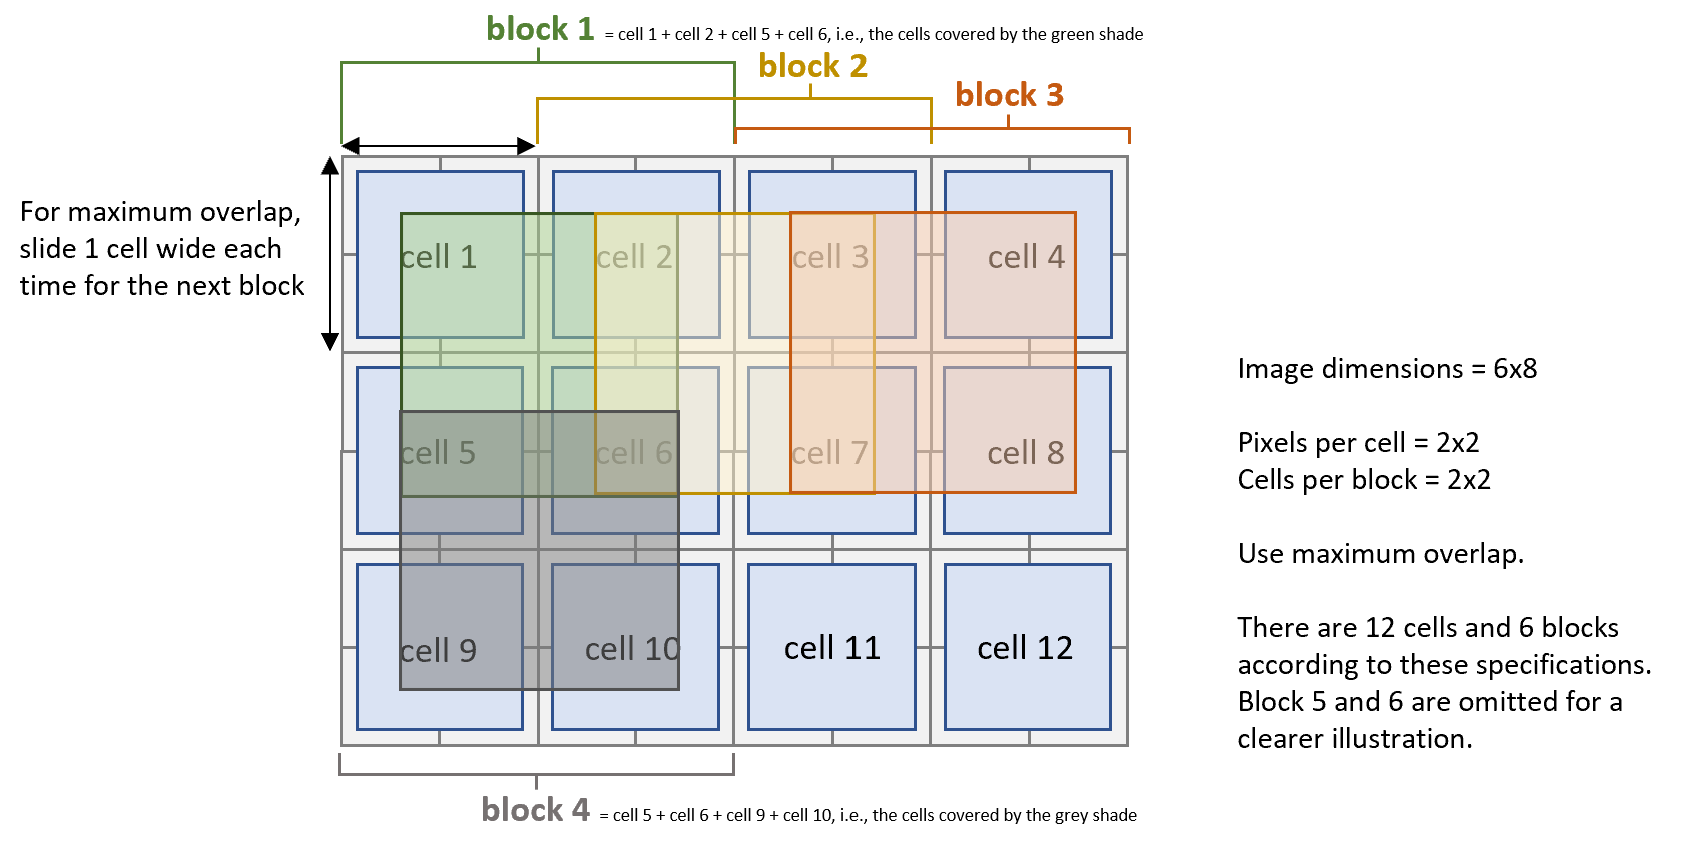
\includegraphics[width=1.3\textwidth]{images/hog-diagram.png}
% \end{center}

\begin{enumerate}[(a)]
\item \textbf{[6 points]}
\begin{tcolorbox}[colback=orange!5!white,colframe=orange!75!black]
     Given a $72\times72$ image, calculate the number of cells, blocks, and final feature vector size that will occur when we extract HOG features over the whole image with the following parameters using maximum overlap between blocks.
\end{tcolorbox}

\begin{enumerate}[(i)]
    \item \textbf{[3 points]} Scenario 1: Pixels per cell = $4\times4$, cells per block = $4\times4$ % (\emph{like in SIFT!}). 

\begin{enumerate}[1.]
    \item \textbf{[1 points]} Number of cells: 
\begin{tcolorbox}[colback=white!5!white,colframe=green!75!black]
        \setbox0=\hbox{\parbox[t]{\textwidth}{
        %%%%%%% ANSWER STARTS HERE %%%%%%%%%%%%%%%%%%%%%%%%%%%%
        
        TODO: Your answer for (a) (i) (1) here
        
        %%%%%%% ANSWER ENDS HERE %%%%%%%%%%%%%%%%%%%%%%%%%%%%%%
        }}
        \clipbox{0pt \dimexpr\dp0-2\baselineskip\relax{} 0in 0pt}{\copy0}
\end{tcolorbox}

    \item \textbf{[1 points]} Number of blocks: 
\begin{tcolorbox}[colback=white!5!white,colframe=green!75!black]
        \setbox0=\hbox{\parbox[t]{\textwidth}{
        %%%%%%% ANSWER STARTS HERE %%%%%%%%%%%%%%%%%%%%%%%%%%%%
        
        TODO: Your answer for (a) (i) (2) here
        
        %%%%%%% ANSWER ENDS HERE %%%%%%%%%%%%%%%%%%%%%%%%%%%%%%
        }}
        \clipbox{0pt \dimexpr\dp0-2\baselineskip\relax{} 0in 0pt}{\copy0}
\end{tcolorbox}

    \item \textbf{[1 points]} Dimensions of feature vector for the whole image: 
\begin{tcolorbox}[colback=white!5!white,colframe=green!75!black]
        \setbox0=\hbox{\parbox[t]{\textwidth}{
        %%%%%%% ANSWER STARTS HERE %%%%%%%%%%%%%%%%%%%%%%%%%%%%
        
        TODO: Your answer for (a) (i) (3) here
        
        %%%%%%% ANSWER ENDS HERE %%%%%%%%%%%%%%%%%%%%%%%%%%%%%%
        }}
        \clipbox{0pt \dimexpr\dp0-2\baselineskip\relax{} 0in 0pt}{\copy0}
\end{tcolorbox}

\end{enumerate}

\item \textbf{[3 points]} Scenario 2: Pixels per cell = $8\times8$, cells per block = $2\times2$.
\begin{enumerate}[1.]
    \item \textbf{[1 points]} Number of cells: 
\begin{tcolorbox}[colback=white!5!white,colframe=green!75!black]
        \setbox0=\hbox{\parbox[t]{\textwidth}{
        %%%%%%% ANSWER STARTS HERE %%%%%%%%%%%%%%%%%%%%%%%%%%%%
        
        TODO: Your answer for (a) (ii) (1) here
        
        %%%%%%% ANSWER ENDS HERE %%%%%%%%%%%%%%%%%%%%%%%%%%%%%%
        }}
        \clipbox{0pt \dimexpr\dp0-2\baselineskip\relax{} 0in 0pt}{\copy0}
\end{tcolorbox}

    \item \textbf{[1 points]} Number of blocks: 
\begin{tcolorbox}[colback=white!5!white,colframe=green!75!black]
        \setbox0=\hbox{\parbox[t]{\textwidth}{
        %%%%%%% ANSWER STARTS HERE %%%%%%%%%%%%%%%%%%%%%%%%%%%%
        
        TODO: Your answer for (a) (i) (2) here
        
        %%%%%%% ANSWER ENDS HERE %%%%%%%%%%%%%%%%%%%%%%%%%%%%%%
        }}
        \clipbox{0pt \dimexpr\dp0-2\baselineskip\relax{} 0in 0pt}{\copy0}
\end{tcolorbox}

    \item \textbf{[1 points]} Dimensions of feature vector for the whole image: 
\begin{tcolorbox}[colback=white!5!white,colframe=green!75!black]
        \setbox0=\hbox{\parbox[t]{\textwidth}{
        %%%%%%% ANSWER STARTS HERE %%%%%%%%%%%%%%%%%%%%%%%%%%%%
        
        TODO: Your answer for (a) (i) (3) here
        
        %%%%%%% ANSWER ENDS HERE %%%%%%%%%%%%%%%%%%%%%%%%%%%%%%
        }}
        \clipbox{0pt \dimexpr\dp0-2\baselineskip\relax{} 0in 0pt}{\copy0}
\end{tcolorbox}

\end{enumerate}
\end{enumerate}

\item \textbf{[4 points]}
When using HOG, the parameters such as pixels per cell and cells per block impact the resulting feature descriptor and so our performance on a classification task.

\begin{tcolorbox}[colback=orange!5!white,colframe=orange!75!black]
    What are the pros and cons of the two parameter combinations? Which might you expect to have better performance? \textbf{[3-6 sentences]}
\end{tcolorbox}

\begin{tcolorbox}[colback=white!5!white,colframe=green!75!black]
        \setbox0=\hbox{\parbox[t]{\textwidth}{
        %%%%%%% ANSWER STARTS HERE %%%%%%%%%%%%%%%%%%%%%%%%%%%%
        
        TODO: Your answer for (b) here
        
        %%%%%%% ANSWER ENDS HERE %%%%%%%%%%%%%%%%%%%%%%%%%%%%%%
        }}
        \clipbox{0pt \dimexpr\dp0-7\baselineskip\relax{} 0in 0pt}{\copy0}
\end{tcolorbox}

\end{enumerate}

%%%%%%%%%%%%%%%%%%%%%%%%%%%%%%%%%%%
% \pagebreak
% \paragraph{A7:} Your answer here.

% \emph{Note: You may find it interesting to read the thesis of Navneet Dalal (co-inventor of HOG) for more information on this topic. \href{http://lear.inrialpes.fr/people/dalal/NavneetDalalThesis.pdf}{[Link to thesis]} (pages 39, 41 in Section 4.3).}


% Uncomment the stencil below and fill in your solution.

% a)
% Scenario 1:
% \\ 
% Number of cells: 
% \\
% Number of blocks: 
% \\
% Dimensions of feature vector for the whole image: 
% \\


% Scenario 2:
% \\ 
% Number of cells: 
% \\
% Number of blocks: 
% \\
% Dimensions of feature vector for the whole image: 
% \\


% What are the pros and cons of the two parameter combinations? Which might you expect to have better performance?
% 

%%%%%%%%%%%%%%%%%%%%%%%%%%%%%%%%%%%



% %%%%%%%%%%%%%%%%%%%%%%%%%%%%%%%%%%%
% \pagebreak
% \paragraph{Secret something to think about:} Given a linear classifier like SVM, how might we handle data that are not linearly separable? How does the \emph{kernel trick} help in these cases? 

% \emph{Hint: See slides in supervised learning crash course deck, plus your own research.}

% %%%%%%%%%%%%%%%%%%%%%%%%%%%%%%%%%%%
% \paragraph{A:} Your answer here.



%%%%%%%%%%%%%%%%%%%%%%%%%%%%%%%%%%%
%%%%%%%%%%%%%%%%%%%%%%%%%%%%%%%%%%%

\pagebreak
\section*{Discussion Attendance:}
\paragraph{Extra Credit:} \textbf{[2 points]}

Please mark this box only if you've attended the discussion session in person.

\begin{tabular}[h]{ll}
$\square$ & I attended the discussion session on DATE \\
\end{tabular}

%%%%%%%%%%%%%%%%%%%%%%%%%%%%%%%%%%%
\pagebreak
\section*{Feedback? (Optional)}
Please help us make the course better. If you have any feedback for this assignment, we'd love to hear it!


% \pagebreak
% \section*{Any additional pages would go here.}

\end{document}